
\newacronym{PEP}{PEP}{Python Enhancements Proposal}
\newacronym{PEPs}{PEPs}{Python Enhancements Proposals}
\newacronym{CI}{CI}{Continuous integration}

Due to the fact that the project team is composed of several developers, who
must review and integrate their work together, it has been necessary to
establish a set of common coding standards.
Besides, because of the open-source nature of the project, the code is
public, and throughout its life will be maintained by multiple developers. For
this reason, a great effort had to be dedicated to ensuring the readability of
the code, along with its documentation, and compliance with strictly established
standards. Among these standards are included two \ac{PEP}, which are the directives that set the different conventions in Python:
the \ac{PEP} 8 - \textit{Style Guide for Python Code}, and the \acs{PEP} 257 - \textit{Docstring Conventions}.

\acs{PEP} 257 documents the semantics and conventions associated with Python
docstrings, which allow include documentation within the code. These docstring
are found next to the code as headers of modules, classes or functions. It has
been used a google-like docstring style, based in the \textit{reStructuredText} format.
This style allows the automatic generation of documentation in pdf and html,
using the \textit{Sphinx} tool. Figure \ref{SBFIG:DOC} shows an extract of the resulting documentation. These pages generated automatically are maintained by
the \ac{CI} system and uploaded to
\href{https://fda.readthedocs.io/}{fda.readthedocs.io}.

%\begin{figure}[Scikit-fda online documentation]{FIG:DOC}{Scikit-fda online documentation}
%  \subfigure[SBFIG:DOC]{Documentation of function}{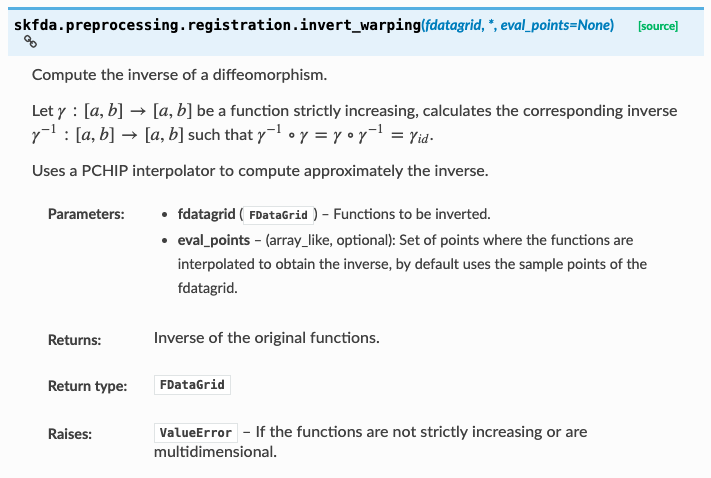
\includegraphics[width=7cm]{doc-a}} \quad
%  \subfigure[SBFIG:DOCTEST]{Doctest included within the documentation}{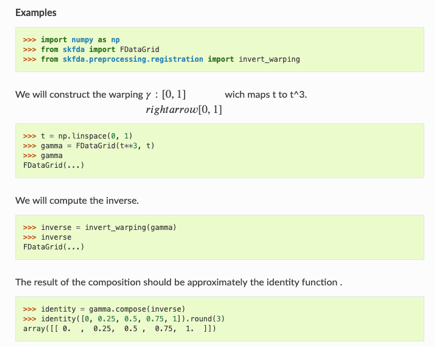
\includegraphics[width=7cm]{doc-b}}
%\end{figure}
\begin{figure}[Scikit-fda online documentation]{SBFIG:DOC}{Scikit-fda online documentation}
	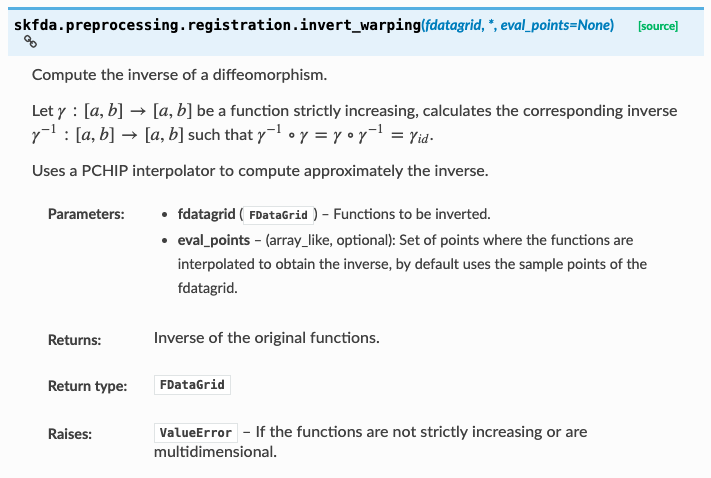
\includegraphics[width=11cm]{doc-a}
\end{figure}

In addition, among the advantages of this kind of documentation is the
possibility of including examples embedded in it, called \textit{doctests}, which appears
 as dynamic short examples within de documentation, as it is shown in the
 Figure \ref{SBFIG:DOCTEST}.
These examples are in turn tests. When running the bench tests, using the tool
pytest, the code is parsed looking for \textit{doctests}, executing the code found in
them and checking that the output matches with the output of the documentation.

\begin{figure}[Doctest]{SBFIG:DOCTEST}{Doctest}
	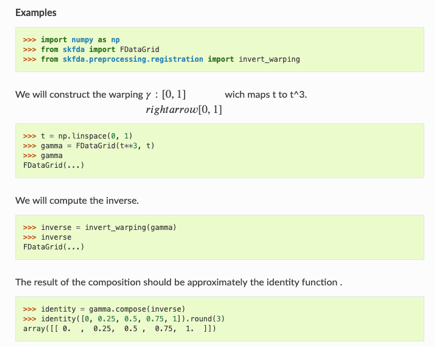
\includegraphics[width=7cm]{doc-b}
\end{figure}

However, the fundamental part of the testing is made up of unit tests, which are
executed together with the \textit{doctests} to check the integrity of the software.
These unit tests check each of the functions developed separately. In order to measure the coverage of these tests, the tool \textit{Coverage} was used, which allows quantifying the lines executed during these tests.

A very relevant part of the package documentation is made up of examples,
which are Python notebooks written as tutorials. Due to their extension, these
examples can be found in Annex \ref{CAP:EXAMPLES} or among the online documentation
at \href{https://fda.readthedocs.io/en/latest/auto_examples/}{fda.readthedocs.io/en/latest/auto\_examples/}.
These examples show simple use cases of the package, linking with the documentation of the functions used. Among the examples created in this work can be found some showing basic functionalities of the representation, such as the composition of functions, interpolation or extrapolation. Examples have also been created by showing the recording techniques mentioned in the Section \ref{SEC:REGISTRATION}, or by using the estimators of nearest neighbours in several simple examples.
